\documentclass[aps,pra,twocolumn,groupedaddress]{revtex4-1}
%\documentclass[12pt]{article}   	% use "amsart" instead of "article" for AMSLaTeX format

\usepackage{amsmath,amssymb}

\usepackage{color}
\usepackage{graphicx}				% Use pdf, png, jpg, or eps� with pdflatex; use eps in DVI mode
								% TeX will automatically convert eps --> pdf in pdflatex		
%\usepackage{caption}
\usepackage{soul}

\usepackage{natbib}
	
\newcommand{\CRout}[1]{\textcolor{blue}{\st{#1}}}
\newcommand{\CR}[1]{\textcolor{blue}{#1}}
\newcommand{\CRcomment}[1]{\textcolor{blue}{\textit{#1}}}

\newcommand{\TBout}[1]{\textcolor{red}{\st{#1}}}
\newcommand{\TB}[1]{\textcolor{red}{#1}}
\newcommand{\TBcomment}[1]{\textcolor{red}{\textit{#1}}}

\newcommand{\PSout}[1]{\textcolor{red}{\st{#1}}}
\newcommand{\PS}[1]{\textcolor{red}{#1}}
\newcommand{\PScomment}[1]{\textcolor{red}{\textit{#1}}}

\begin{document}

\title{Hydrodynamic analogues of quantum theory in a bouncing droplet system}
%\author{Chris Richardson, Peter Schlagheck, John Martin, Nicolas Vandewalle, Thierry Bastin}
% \affiliation{\CR{D\'epartement} de Physique, University of Liege, 4000 Liege, Belgium}
%\address{\CR{D\'epartement} de Physique, \affiliation{University of Liege}, 4000 Liege, Belgium}
\author{Chris D. Richardson}
\author{Peter Schlagheck}
\author{John Martin}
\author{Nicolas Vandewalle}
\author{Thierry Bastin}
\affiliation{D\'epartement de Physique, University of Liege, 4000 Liege, Belgium}
\date{\today}							% Activate to display a given date or no date

\begin{abstract}

Empty

\end{abstract}

\maketitle

\section{Introduction}

A liquid droplet bouncing on a vibrating bath can be made to persist bouncing indefinitely~\cite{PhysRevLett.94.177801}.  The droplet is given a vertical velocity by due to the action of the vibrating bath, assuming the force is large enough to counteract gravity.  Upon landing the droplet will avoid coalescing into the bath if the impact time is less than what is required for the air layer between the droplet and the bath to decay.  Therefore the droplet will get another kick from the bath and this cycle repeats in perpetuity and the bouncing period is directly related to the frequency of the vibrator.  The effect of these oscillatory bounces on the bath is the production of radial standing waves, Faraday waves, centered on the position of the droplet at each impact.  These waves persists over many bounces of the droplet~\cite{FLM:8266690} due to the energy imparted to them by the vibrator.  This effect is referred to as the memory since the bath will in effect memorize, in the form of persistent Faraday waves, the impacts of many bounces of the droplet.  This memory parameter is directly related to the amplitude of the bath's vibration.  It ranges from zero with a zero vibration amplitude up to infinity to closer the amplitude the vibration comes to what is called the Faraday threshold.  This threshold is the point at which the liquid surface stops being flat in the absence of perturbations other than the vibrator.  Vibrating the bath above the faraday threshold will cause a regular wave pattern of upon the bath's surface.  If, however, the bath is vibrated near, but not over, the Faraday threshold, a droplet with a constant velocity, called a walker, can be formed~\cite{CouderWalkingNature}.  

The walking droplet is particularly interesting as it is propelled by the surface wave that it itself creates.  It is therefore natural to explore the motion of the droplet when the surface wave is modified in some way either through interaction with the environment or the presence of another droplet.  This has been the focus of many experiments and it has been noted that the behavior of these droplets is analogous to the behavior of particles in quantum mechanics.  Specifically we have seen... [insert reference storm].

The droplets path being guided by a surface wave is reminiscent of the de Broglie-Bohm pilot wave interpretation interpretation of quantum mechanics in which a quantum particle is guided by a wave function, a comparison which has been often noted[cites] and which we will continue to explore.  In the de Broglie-Bohm interpretation particles have no properties other than position.  The evolution of these particles is completely determined by the wave function and the guiding equation.  The wave function evolves according to Schr\"odinger's equation and the particles equation of motion uses the wave function as input to a first order guiding differential equation proportional to the probability current.  In actuality de Broglie initially had a slightly different pilot wave model than the traditional de Broglie-Bohm pilot wave model popular today.  De Broglie used a two solution model in which both the particle and the wave obeyed separate wave equations.  In this model the particle had a frequency analogous to a de Broglie wavelength and it was the interaction of the particles wave with the wave function which led to the motion of the particle.  It is obvious why this model might be attractive to those dealing with the bouncing droplet system as the droplet creates its own surface wave which is analogous to a particle with a de Broglie wavelength.  Unfortunately de Broglie's two solution model was never completed it is therefore unsuitable as a comparative model and we must use the de Broglie-Bohm model.  To make a comparison to a classical system, such as the droplet bouncing system, the guiding equation can be reinterpreted as a potential, Bohm's quantum potential, in traditional Newtonian mechanics.  The force due to this potential gives rise to all the uniquely quantum behavior seen in quantum systems and it is this force in which we use make comparisons with the bouncing droplet system.

Here we focus on these hydrodynamic analogues of quantum mechanics, explore their origin, and determine to what extent these analogies hold.  We do this by first describing the bouncing droplet system in the language of pilot wave theory and then comparing the behavior to a similar quantum system in the framework of the de Broglie-Bohm pilot wave model[cite].  This comparison requires two things, a description of the force on the particle and a description of the wave that gives rise to that force.  The hydrodynamic force on a droplet is known and it merely falls to us to make the analogy to the force from Bohm's quantum potential.   We then describe the excited Faraday surface waves produced by a walking droplet, transform it into the continuous domain, and explore the analogies to a Bohmian pilot wave.  We then use this model to explore the single and double slit experiments and use the results to comment on what analogies can be made to the results of the quantum experiments and to what extent those analogies hold.  We also, in the spirit of Bohmian mechanics, explore the consequences of separating the generator of the guiding wave from the droplet by associate it instead with the experiment.

\section{The hydrodynamic model}

\subsection{The force on a droplet}

In Bohm's formulation of the pilot wave model, the quantum potential is complementary to Schr\"odinger's equation (see the Madelung transformation)[cite] and little effort is required to motivate it.  However, in the bouncing droplet system, where the droplet and wave are both macroscopically distinct entities,  it is not clear that the source of the force on the particle flows from a convenient differential equation such as Schr\"odinger's.  It is, however, well known~\cite{FLM:431290,bib:CouderSingle,CouderWalkingNature} that the droplet's velocity between bounces will change in proportion to the angle, $\theta$, of the surface wave at the point where the droplet impacts it.  We can therefore follow Couder and Fort~\cite{1742-6596-361-1-012001} and write the change of velocity and position of a walking droplet after the $n$th impact as

\begin{align}
\Delta \dot{\mathbf{r}} &\propto -  \left( \sin(\theta_x) \hat{x} + \sin(\theta_y) \hat{y} \right) \propto -  \nabla \zeta_{n}(\mathbf{r}) \label{eqn:CoudersPot} \\
\Delta \mathbf{r} &\propto \dot{\mathbf{r}}_n
\end{align}
where $T_F$ is the Faraday frequency, the period of one bounce which is half the forcing frequency, and $\zeta_{n}(\mathbf{r})$ is the amplitude of the surface wave at the $n$th bounce.

The force on the droplet is then
\begin{align}
m \ddot{\mathbf{r}}_{n} &=m \frac{\Delta \dot{\mathbf{r}}}{T_F}  \propto  - \nabla \zeta_{n}(\mathbf{r})
\end{align}
We now move into the continuous domain where $\ddot{\mathbf{r}}_{n} \rightarrow \ddot{\mathbf{r}}$.  
\begin{align}
m \ddot{\mathbf{r}} &= - F_d \nabla \zeta_{\textrm{eff}}(\mathbf{r},t) \label{eqn:newforce}
\end{align}
where $F_d$ is... and $\zeta_{\textrm{eff}}$ is...

Motivated by the model due to [cite] we add a viscous damping term proportional to velocity that is necessary to avoid unrealistically large velocities for the droplet.
\begin{align}
m \ddot{\mathbf{r}} &= - F_d \nabla \zeta_{\textrm{eff}}(\mathbf{r},t) - f^V \dot{\mathbf{r}} \label{eqn:newforce_damp}
\end{align}

\subsection{The excited wave of a walker}

\begin{figure}[ht]
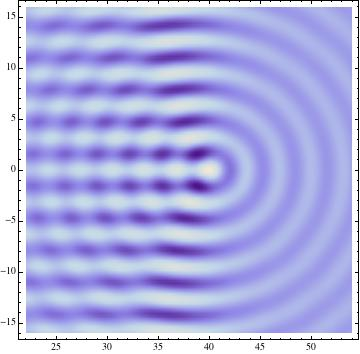
\includegraphics[width=1\linewidth]{Graphics/WaveFront3D.jpg}
\caption{The surface wave is a combination of excited Faraday waves due to many bounces of a droplet with a constant velocity and exponential damping in time.}
\label{fig:WaveFront3D}
\end{figure}

Consider a walking droplet bouncing on a vibrating surface where the constant[cite] speed of the droplet, $v_d = \frac{\Delta r}{T_F}$, typically on the order of $v_d \approx \omega_F / (10 k_F) \approx 10 mm / s$[cite].  This velocity is much less that the speed of the expanding wave produced by the impact of the droplet which is on the order of [what?].   This allows us to ignore the expansion and approximate the the excited Faraday wave by an oscillating Bessel function exponentially damped in time~\cite{FLM:8266690,0295-5075-102-1-16005}
\begin{align}
\zeta(\mathbf{r},t) = A \cos(\omega_F t)  J_0\left(k_F  |\mathbf{r} - \mathbf{r}_0 | \right) e^{- (t-t_0)/\tau} \label{eqn:damped_intitial}
\end{align}
where the damping parameter $\tau = T_F M$ is determined by the angular frequency, $\omega_F = 2 \pi / T_F$, of the excited Faraday waves which is typically an the order of $2 \pi 20 Hz$, the wave number, $k_F$, is on the order of $2 \pi / 5.55 mm \approx 1 radian / mm$,  $M$ is the dimensionless memory parameter which is a measure of the distance to the Faraday threshold and roughly equivalent to the number of impact waves the bath will store.  

[rephrase] This form of the excited Faraday effectively makes the wave nonlocal with respect to the droplet which is analogous to the wavefunction in quantum mechanics or the pilot wave in the de Broglie-Bohm interpretation which are both manifestly nonlocal.  This is an important point in that it allows the excited Faraday wave to be effected by distant perturbations which in turn will effect the path of the droplet in an effectively nonlocal manner.  

The walking droplet bounces in sync with the vibrator~\cite{CouderWalkingNature} and therefore only interacts with the surface wave stroboscopically.  At every bounce the time dependent part of the excited wave is changed by $\Delta t = T_F =\frac{2 \pi}{\omega_F}$ and we can discretize the time into only the times in which the droplet interacts with the bath, $t_n = n \Delta t$.  We can, therefore, drop the value of the time dependent part of Eq.~\ref{eqn:damped_intitial}, $\cos(\omega_F t_n) = \cos(2 \pi) = 1$.  The first excited Faraday wave as of yet undamped by the memory parameter is then
\begin{align}
\zeta_0(\mathbf{r}) = A J_0\left(k_F  |\mathbf{r} - \mathbf{r}_0 |  \right) \label{eqn:damped_intitial_strob}
\end{align}

In the walking regime the droplet moves at a constant velocity an amount $\Delta \mathbf{r}$ over the period $T_F$.  Therefore, the next standing wave produced by the second impact of the droplet is an excited wave at the new position of the droplet and the previous excited wave damped due to the memory parameter
\begin{align}
\zeta_1(\mathbf{r}) &= \zeta_0(\mathbf{r}) e^{- t_1/\tau} +  A J_0\left(k_F |\mathbf{r} - \mathbf{r}_1 | \right)
\end{align}
where $\mathbf{r}_1 = \mathbf{r}_0 -  \Delta \mathbf{r}$. The resulting waves that add up after $N$ bounces create and combined wave
\begin{align}
\zeta_{N}(\mathbf{r}) &= A \sum\limits_{n=0}^N J_0\left(k_F |\mathbf{r} - \mathbf{r}_n | \right) e^{-(t_N - t_n)/\tau} \label{eqn:exactsum}
\end{align}
where $t_N = N T_F$ is equal to the total evolution time of the droplet, and $\mathbf{r}_n = \mathbf{r}_0 - n \Delta \mathbf{r}$.  This is a similar equation as the the one given in~\cite{FLM:8266690,Fort12102010} where we differ by not using the asymptotic expansion of the Bessel function and not having a spatial damping term due to the viscosity of the fluid.  As can be seen in Fig.~\ref{fig:WaveFront3D} this gives the expected horseshoe shaped wave traveling at the speed of the droplet with a wavelength determined by the oscillator.  The shape of the wave behind the droplet is quite complex but this complexity can be avoided by looking only at the forward part of the effective wavefunction which is the strategy we employ in our double slit example below.

Let us look ahead and consider the portion of the effective wave function which impinges on a double slit when the droplet is still a large distance away from those slits.  In this limit, $|\mathbf{r} - \mathbf{r}_n| =  |\mathbf{r} - \mathbf{r}_N + (N-n) \Delta \mathbf{r}| \approx |\mathbf{r} - \mathbf{r}_N| + (N-n) |\Delta \mathbf{r}| \cdot \frac{\mathbf{r} - \mathbf{r}_N}{|\mathbf{r} - \mathbf{r}_N|} + \mathrm{O}(|\Delta \mathbf{r}|^2)$ and the effective wave is

\begin{align}
\zeta_{N}(\mathbf{r}) &= A \sum\limits_{n=0}^N  J_0\left(k_F  |\mathbf{r} - \mathbf{r}_N + (N-n) \Delta \mathbf{r}| \right)  e^{-(N - n) \Delta t / \tau} \\
&\approx \frac{A}{2 \pi} \int^{\pi}_{-\pi} e^{i k_F  |\mathbf{r} - \mathbf{r}_N|  \sin \phi } \notag d\phi \\
&\times \sum\limits_{n=0}^N   e^{i k_F (N-n) | \Delta \mathbf{r} |  \cdot \frac{\mathbf{r} - \mathbf{r}_N}{|\mathbf{r} - \mathbf{r}_N|}   \sin \phi }  e^{-(N - n) \Delta t / \tau}
\end{align}
If we note that far from the droplet $| \Delta \mathbf{r} |  \cdot (\mathbf{r} - \mathbf{r}_N) \approx 0$ we can write the effective wave as a Bessel function which travels in discrete steps
\begin{align}
\zeta_{N}(\mathbf{r}) &\approx \tilde{A} J_0( k_F  |\mathbf{r} - \mathbf{r}_N| ) 
\end{align}
where $\tilde{A}$ is... We assume [what?] and move into the continuous domain with $t_N \rightarrow t$ and $\mathbf{r}_N \rightarrow \mathbf{r}_d(t) =  \frac{t}{T_F} \Delta \mathbf{r}$ giving
\begin{align}
\zeta_{\textrm{eff}}(\mathbf{r}, t) &\approx \tilde{A} J_0\left(k_F  |\mathbf{r} - \mathbf{r}_d(t)| \right)  \label{eqn:travelingWave} 
\end{align}

\subsection{Analogues in the equations}

\begin{figure}[ht]

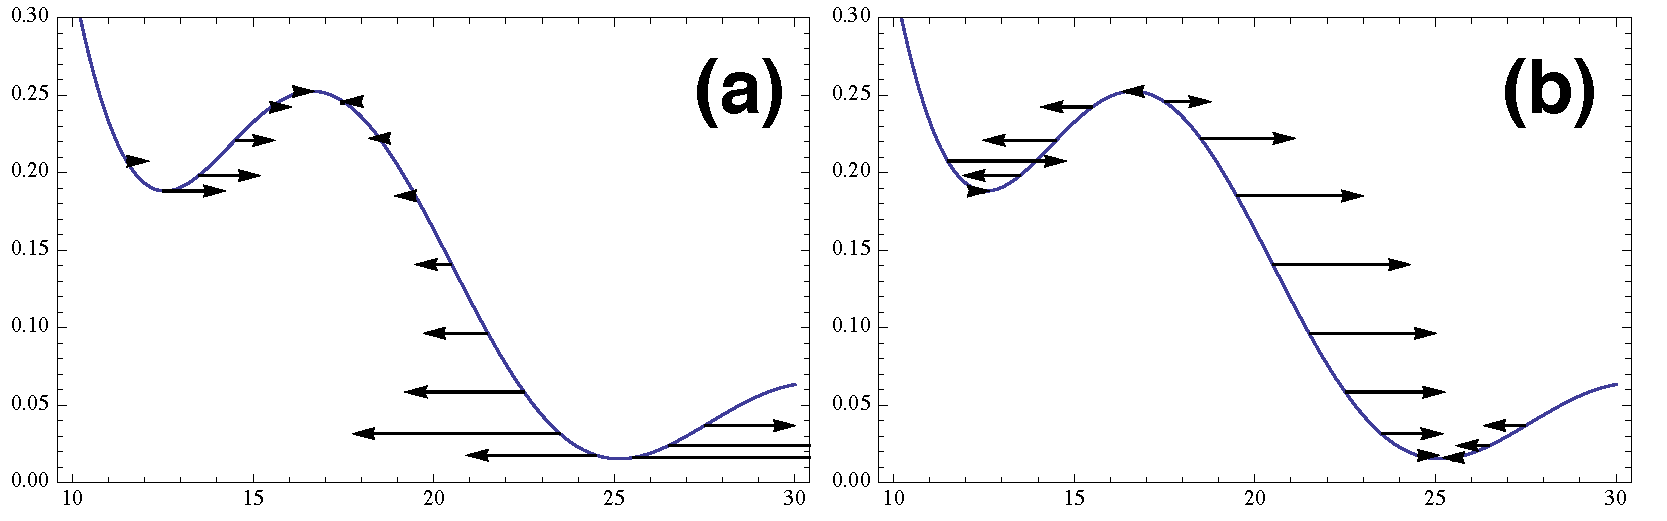
\includegraphics[width=1\linewidth]{Graphics/CombinedGraphics/ForceComparison}
\caption{Relative magnitudes and direction of the force on a quantum particle calculated from Bohm's quantum potential along an arbitrary probability density.  At the points the probability is zero the force on the particle is infinite.  Magnitudes and direction of the force on a droplet calculated from hydrodynamic force along an arbitrary surface wave.  The droplet is encouraged to move towards and remain in the trough of the wave.}
\label{fig:ForceComparison}

\end{figure}

We can now explore to what extent the force on a droplet due to a surface wave is analogous to the force on a quantum particle due to quantum wave function.  [first order?]  If we define the combined wave due to many bounces of the droplet as the \emph{effective potential} $U_{\textrm{eff}} = m g \zeta_{\textrm{eff}}$, we can make a direct comparison to Bohm's quantum potential, $U_q(\mathbf{r},t)$, and the resultant Newtonian force given by
 \begin{align}
U_q(\mathbf{r},t) &= - \frac{\hbar^2}{2 m} \frac{\nabla^2 \left| \psi(\mathbf{r},t) \right|}{\left| \psi(\mathbf{r},t) \right|} \\  \label{eqn:qmp}
m \ddot{\mathbf{r}} &= - \nabla U_q(\mathbf{r},t)
\end{align}
To demonstrate the differences between the two cases, we explore a slice of a quantum probability density shown in Fig.~\ref{fig:ForceComparison}-A and an identical slice of an effective potential Fig.~\ref{fig:ForceComparison}-B and graph the magnitude and direction of the force on the quantum particle or droplet.  When looking at the behavior of the quantum force when the wavefunction is close to zero, the quantum force is singular whereas the effective hydrodynamic force is not.  There is a very strong quantum mechanical force that will move a particle away from an area of low probability as can be seen in Fig.~\ref{fig:ForceComparison}-A.  Conversely our force directs the droplet into the trough of the wave as can be seen in Fig.~\ref{fig:ForceComparison}-B.  There is also an unstable equilibrium point as the crest of the wave which is absent with Bohm's quantum force.

Having said this, we should note that even though the source of both the Bohmian force and our hydrodynamic force are not mathematically or functionally equivalent to their quantum counterparts, a probabilistic  analogy can still be made.  The effect of the the forces from the two guiding equations is analogous if we consider those areas of the effective wavefunction with large slope to be equivalent to areas of low probability in the quantum wavefunction.  Both forcing equations apply a strong force that will remove a particle from an area of low probability (high slope).  Further, because the force and likely therefore the velocity of the droplet in an area of high slope (low probability) is high, the droplet will spend less time in that area and be therefore less likely to be found.

\section{The slits}

Following Feynman we ``choose to examine a phenomenon which is impossible, absolutely impossible, to explain in any classical way, and which has in it the heart of quantum mechanics. In reality, it contains the only mystery.''[cite].  He is, of course, speaking about the self interference of a particle through one or more slits.  This well known phenomenon has a direct an analogue in the bouncing droplet system as observed by Couder[CITE].  We submit, however, that even though interference in the bouncing droplet system is analogous to the interference seen in quantum mechanics, the mechanism of that interference is quite different and care should be taken with to what extent the analogy is valid.  Because we have developed an effective surface wave and a guiding equation, we can demonstrate the similarities and differences to quantum mechanics by examining the bouncing droplet system in light of the single and double slit experiments.

We have from Eq.~\ref{eqn:travelingWave} a simple surface wave traveling at the speed of the droplet, $v_d$.  We can send this wave through one or more slits.  When the droplet is still far from the slit, the wave impinging on the slit(s) is approximately a plane wave and it is then well known through a simple application of Huygen's principle what the wave pattern will be after the slit(s).  We approximate the wave after the slits by filling the slits with emitters of circular waves with the same wave number and frequency as the stroboscopic surface wave excited by the droplet, Eq.~\ref{eqn:travelingWave}.  We define the angular frequency of these waves as $\omega_d = k_F v_d$ and write the surface wave emanating from one slit as
 \begin{align}
\zeta_{\textrm{eff}}(\mathbf{r}, t) &= \Lambda \frac{1}{L} \sum\limits_{l=0}^L Re \left[e^{-i \omega_d t} H_0^{(1)} (k_F |\mathbf{r} - \mathbf{r}_l |)\right]  \label{eqn:huygens}  
\end{align}
where $\mathbf{r}_l$ for $0 < l< L$ spans the space of the slit, $\Lambda$ is the amplitude of the wave, and $H_0^{(1)}$ is the outgoing Hankel function.  [talk about $\Lambda$] The result of which can be seen in Fig.~\ref{fig:SingleSlitDensitiesAndTrajectories}-B.  This will be the surface wave beyond a slit until the droplet gets close to the slit and we can no longer assume the parallel wave approximation in Eq.~\ref{eqn:travelingWave}.  However, if we work in the high memory regime, $M > 100$, we notice that the contribution to the post-slit wave by the droplets excited surface wave when the droplet is close to the slit (out of the regime in which Eq.~\ref{eqn:travelingWave} is valid) is small in comparison to the contribution to the post-slit wave by the droplets excited surface wave when the droplet is far from the slit (where Eq.~\ref{eqn:travelingWave} is valid).  The contributions to the wave when the droplet is far from the slit, which occur over a long time, obscures the contributions when the droplet is near the slits, which occur over a relatively short time.  And so, in the high memory regime, the wave after the slits can still take the relatively simple form of Eq.~\ref{eqn:huygens}.

While it is necessary for us to work in the high memory regime it is important not to ignore the memory effect all together.  After the droplet passes through the slit the post-slit surface wave will begin to degrade since it is no longer being reinforced by waves coming through the slit.  Also when the droplet passes the slit the droplet begins to add its own excited wave to the degrading post-slit surface wave already present.  Because of this we limit our observations of the droplet after the slit to $100 T_F$, inside the high memory regime, where the post-slit surface wave is still dominant compared to the continuing contributions from the droplet.

\subsection{The single slit}

\begin{figure}[ht]
 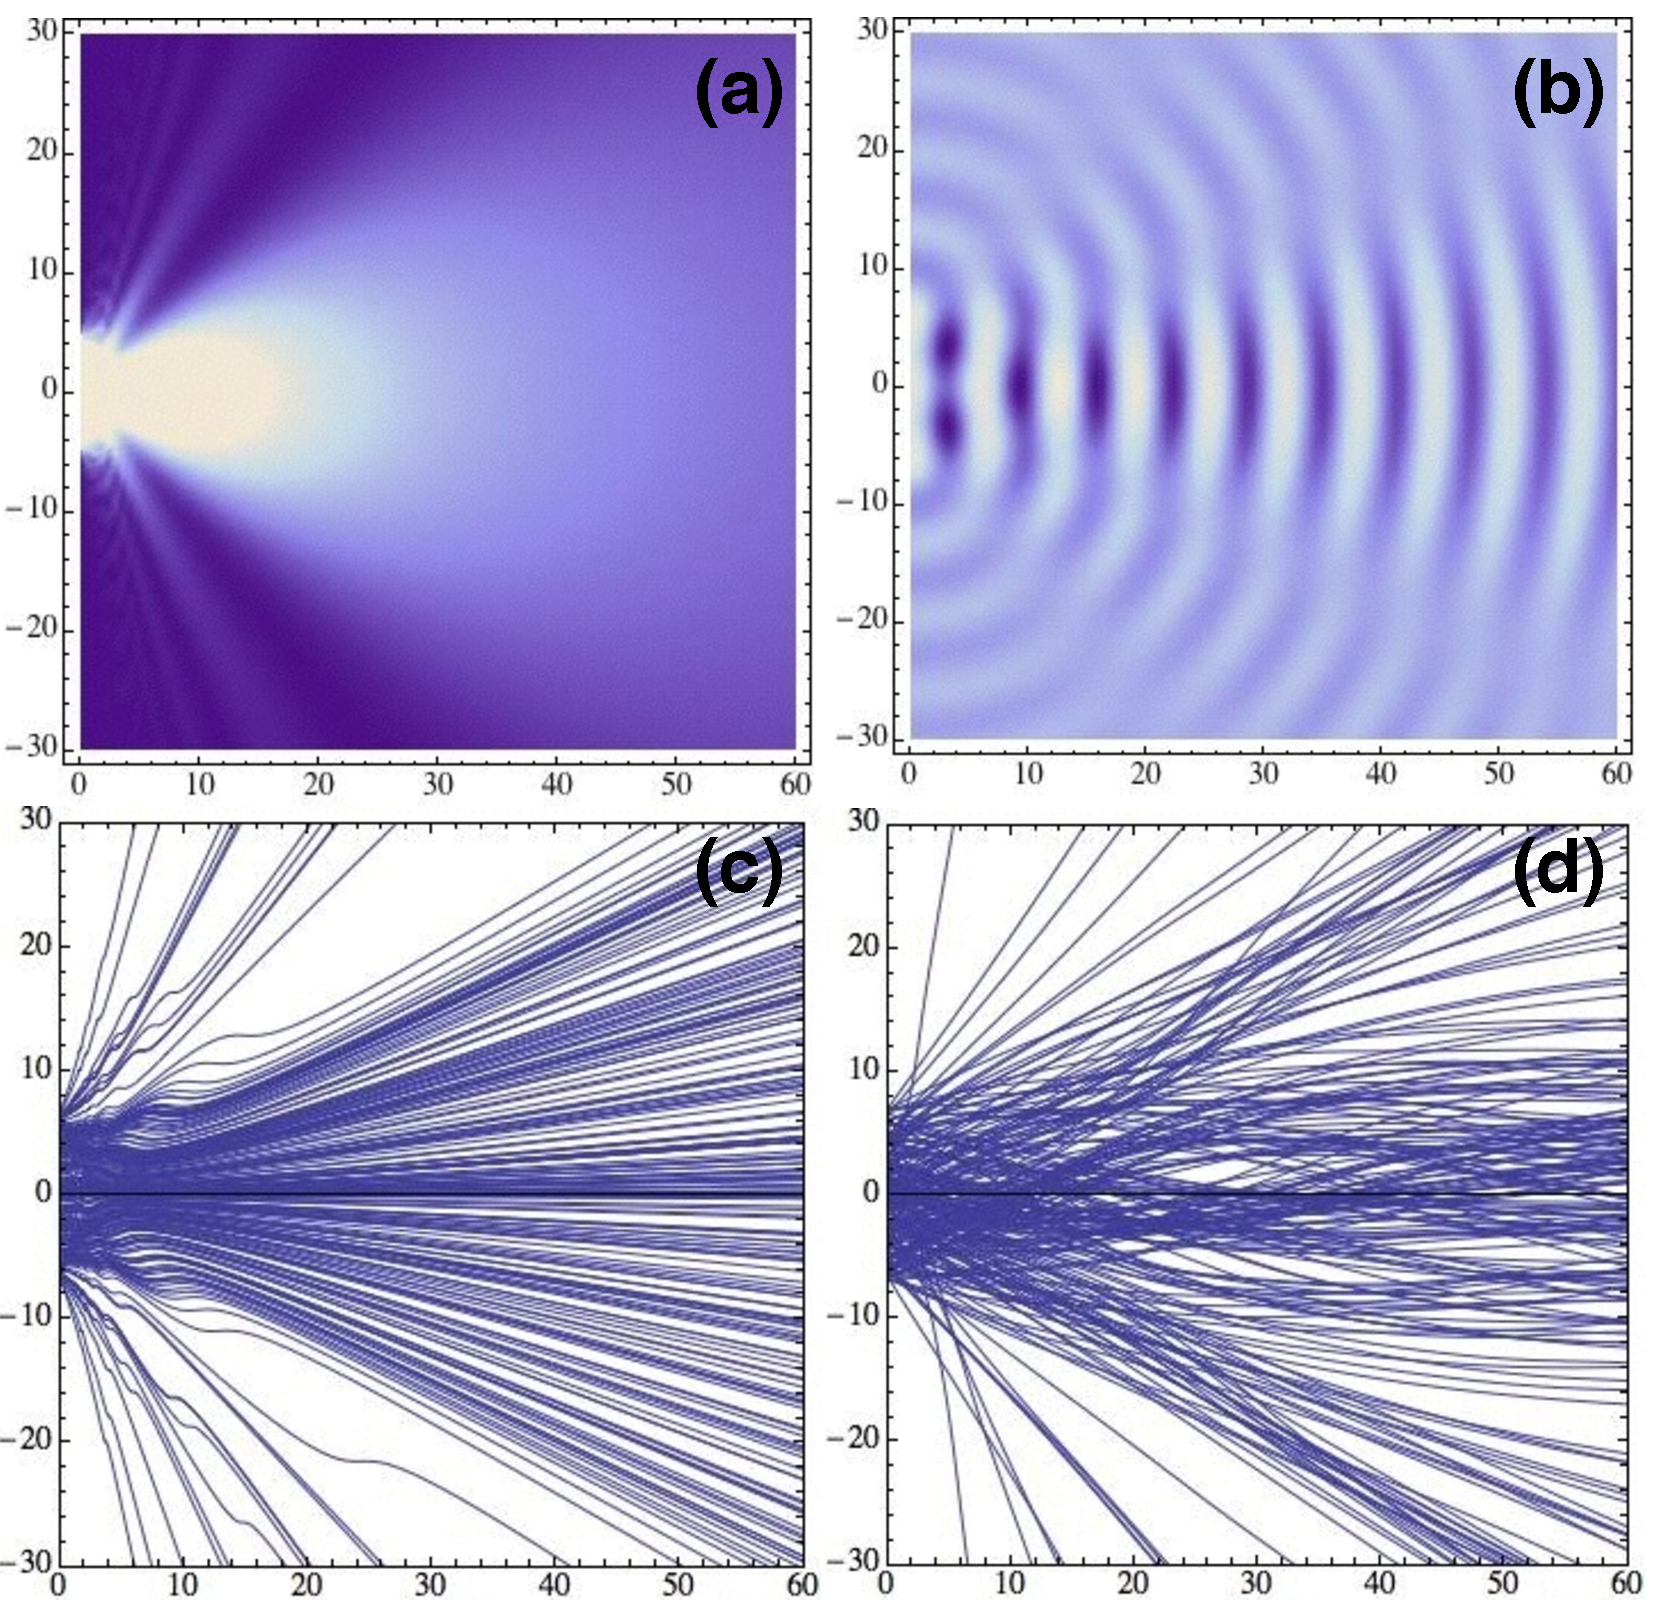
\includegraphics[width=1\linewidth]{Graphics/CombinedGraphics/SingleSlitDensitiesAndTrajectories}
\caption{(A)Density plot of the probability density of a quantum particle passing through two slits a distance 5mm apart with a gaussian slit width of width 1mm.  (B)Density plot of the surface wave of the bath after the droplet wave has passed through a slit  of width 8mm.  (C)Trajectories due to Bohm's quantum potential of many quantum particles passing through two slits a distance 5mm apart with a gaussian slit width of width 1mm.  (D)Trajectories due to the hydrodynamic force  of many droplets passing through two slits a distance 5mm apart with a gaussian slit width of width 1mm.}
\label{fig:SingleSlitDensitiesAndTrajectories}
\end{figure}

\begin{figure}[ht]
 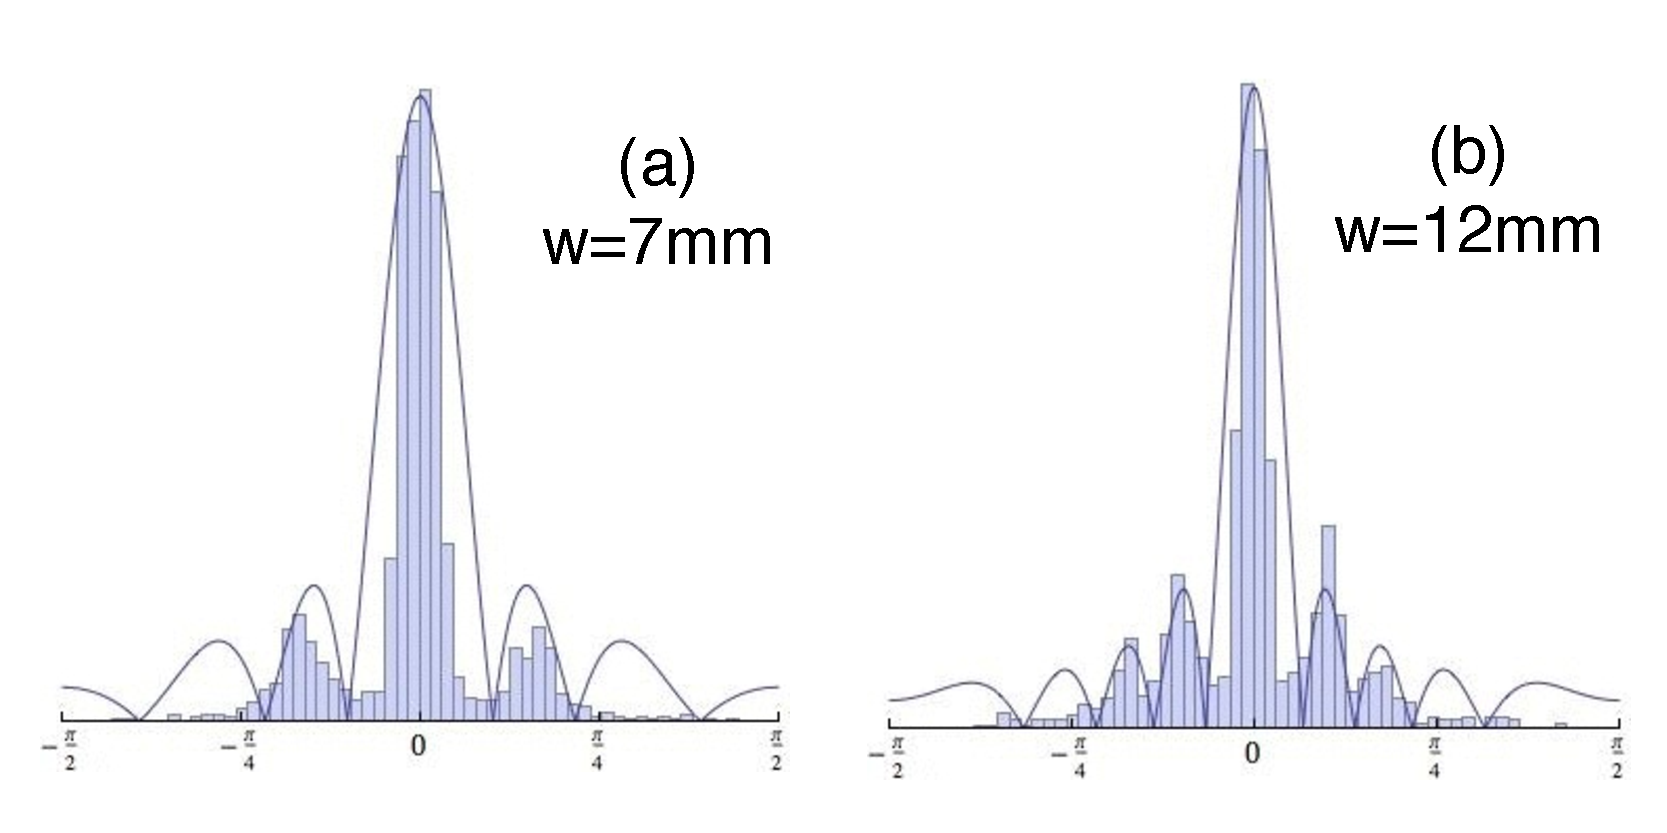
\includegraphics[width=1\linewidth]{Graphics/CombinedGraphics/SingleSlitHistWidths}
\caption{empty}
\label{fig:SingleSlitVisibilityHistograms}
\end{figure}

[I think a figure which shows the histograms for the Bohmian case, and three other cases with varying slit widths is appropriate.]

Using Eq.~\ref{eqn:huygens} with Eq.~\ref{eqn:newforce_damp}  we numerically compute the paths followed by many droplets with initial positions distributed uniformly along the slit, the initial angle of velocities $cos$ distributed, and the magnitude of the initial velocity equal to that of the walking droplet, $v_d$.  The results shown in Fig.~\ref{fig:SingleSlitDensitiesAndTrajectories}-D can be contrasted to the trajectories in Fig.~\ref{fig:SingleSlitDensitiesAndTrajectories}-C, which are the result of the quantum wavefunction and Bohm's quantum force.  They are fundamentally different but sure some traits in the broad sense.  If we look at the matching histogram given by Fig.~\ref{fig:SingleSlitVisibilityHistograms}-B we note that the interference pattern that builds gives similar results to that of the quantum case even though the trajectories are quite dissimilar.  Mathematically and physically the droplet system is far rom being quantum, but the experiment gives similar statistical results.  [Couder's results]

\subsection{The double slit}

\begin{figure}[ht]
 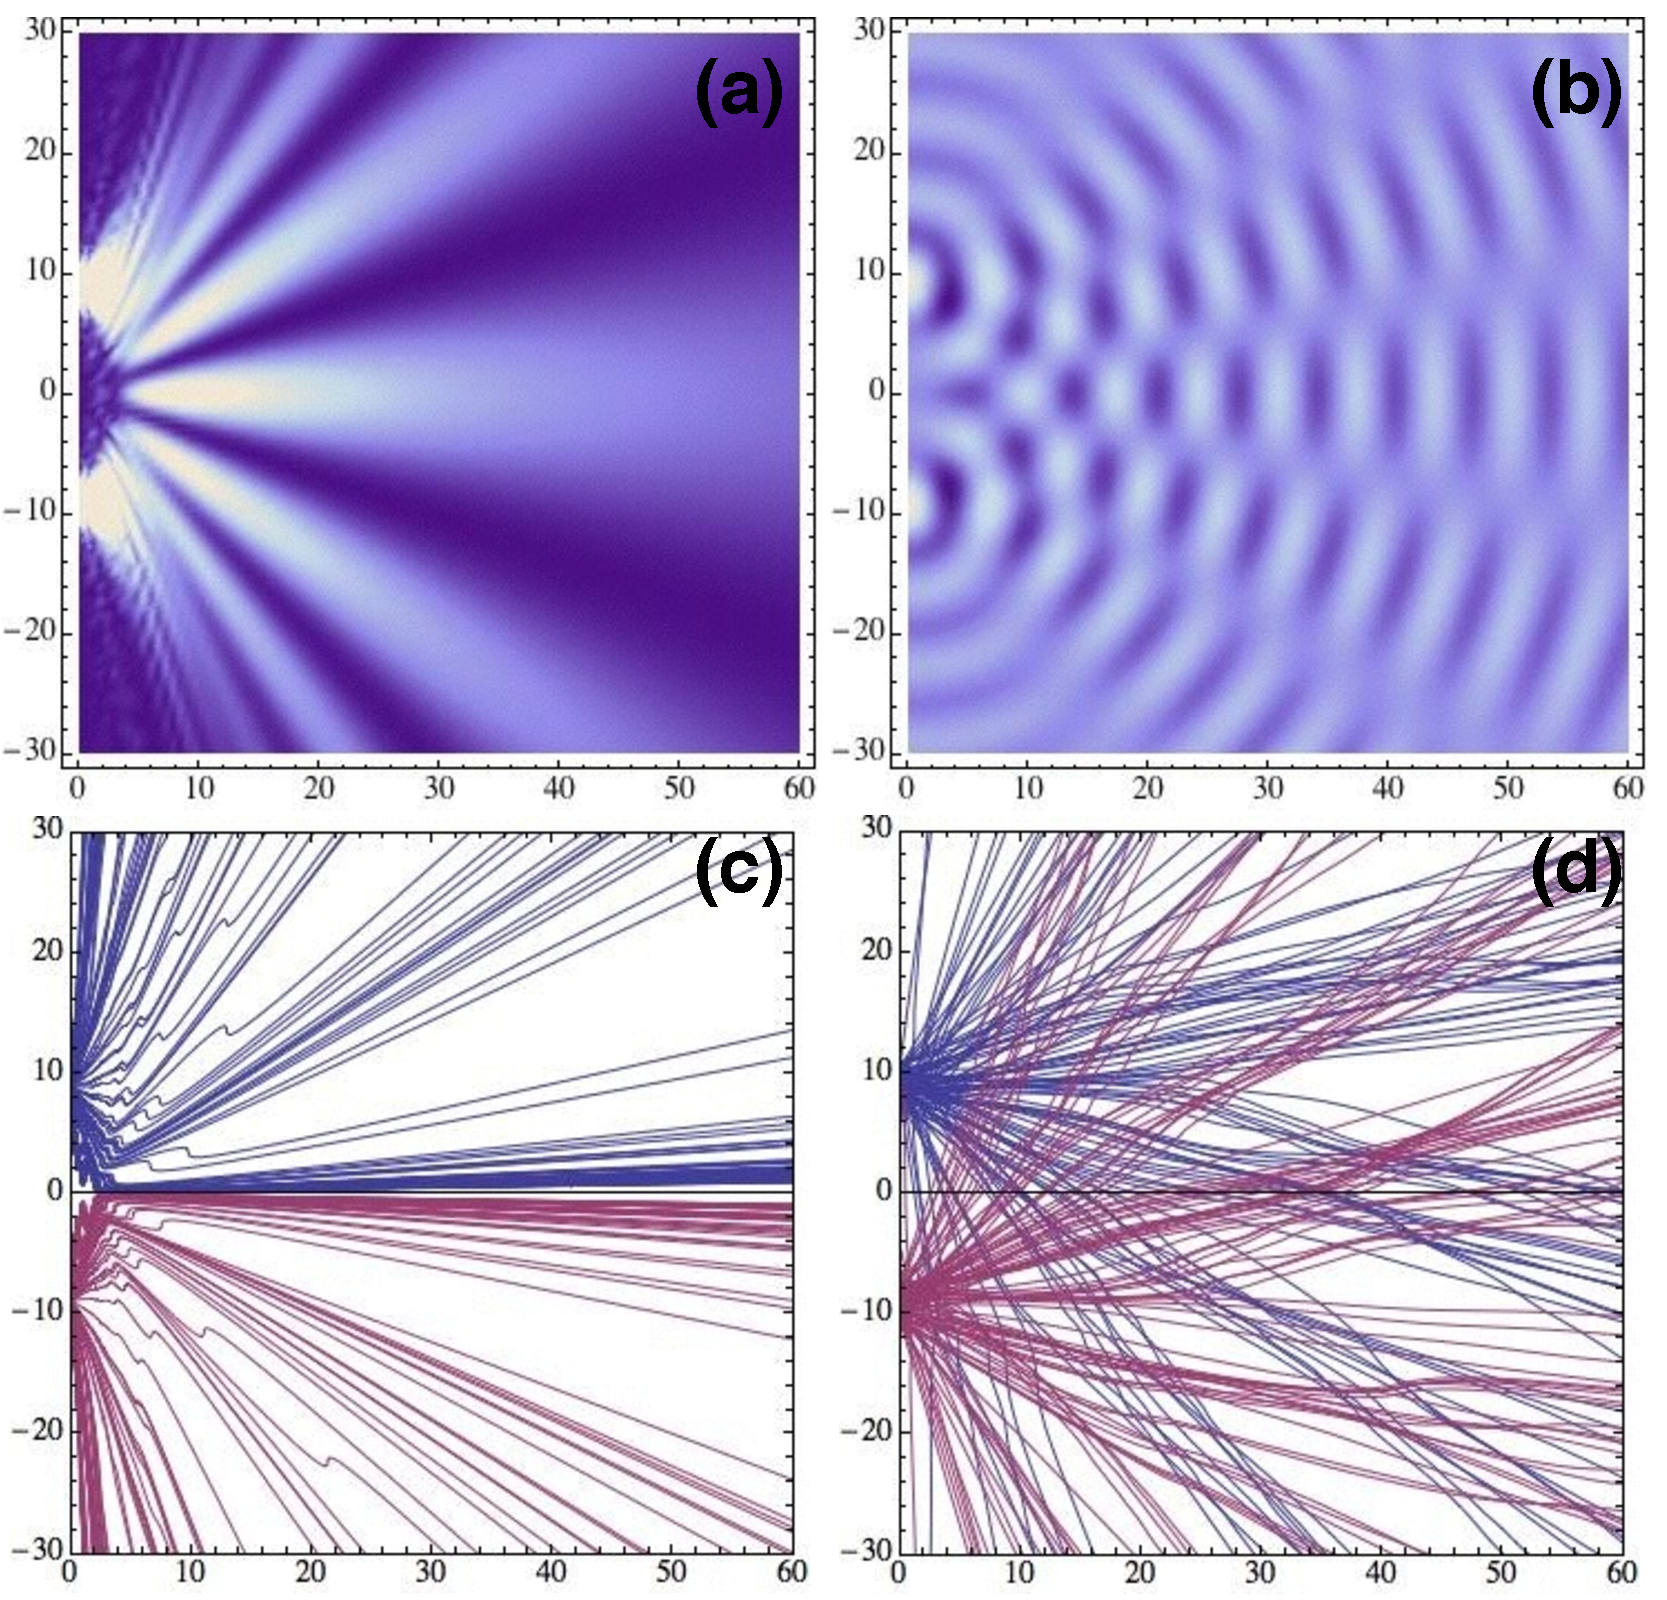
\includegraphics[width=1\linewidth]{Graphics/CombinedGraphics/DoubleSlitDensitiesAndTrajectories}
\caption{Plots for the double slit experiment with slits of width 1mm a distance 5mm apart.  Here $v_d \approx 10 mm/s$, $k_F = 2 \pi / \lambda_F = 2 \pi / (5.5 mm) \approx 1 radian / mm$, $\omega_d = k_F v_d \approx 10 radian / s$, the distance it takes a free space walker to bounce 100 times is $L(M) = v_d M T_F = 10 mm/s * 100 * 0.04 s = 40 mm$.  (a)Density plot of the probability density of a quantum particle where the initial distribution of particles is gaussian distributed with a width equal to the 1mm.  (b)Density plot of the surface wave of the bath after the droplet wave has passed through the two slits.  (c)Trajectories due to Bohm's quantum potential of many quantum particles passing through two slits.  (d)Trajectories due to the hydrodynamic force of many droplets passing through the two slits.}
\label{fig:DoubleSlitDensitiesAndTrajectories}
\end{figure}

\begin{figure}[ht]
 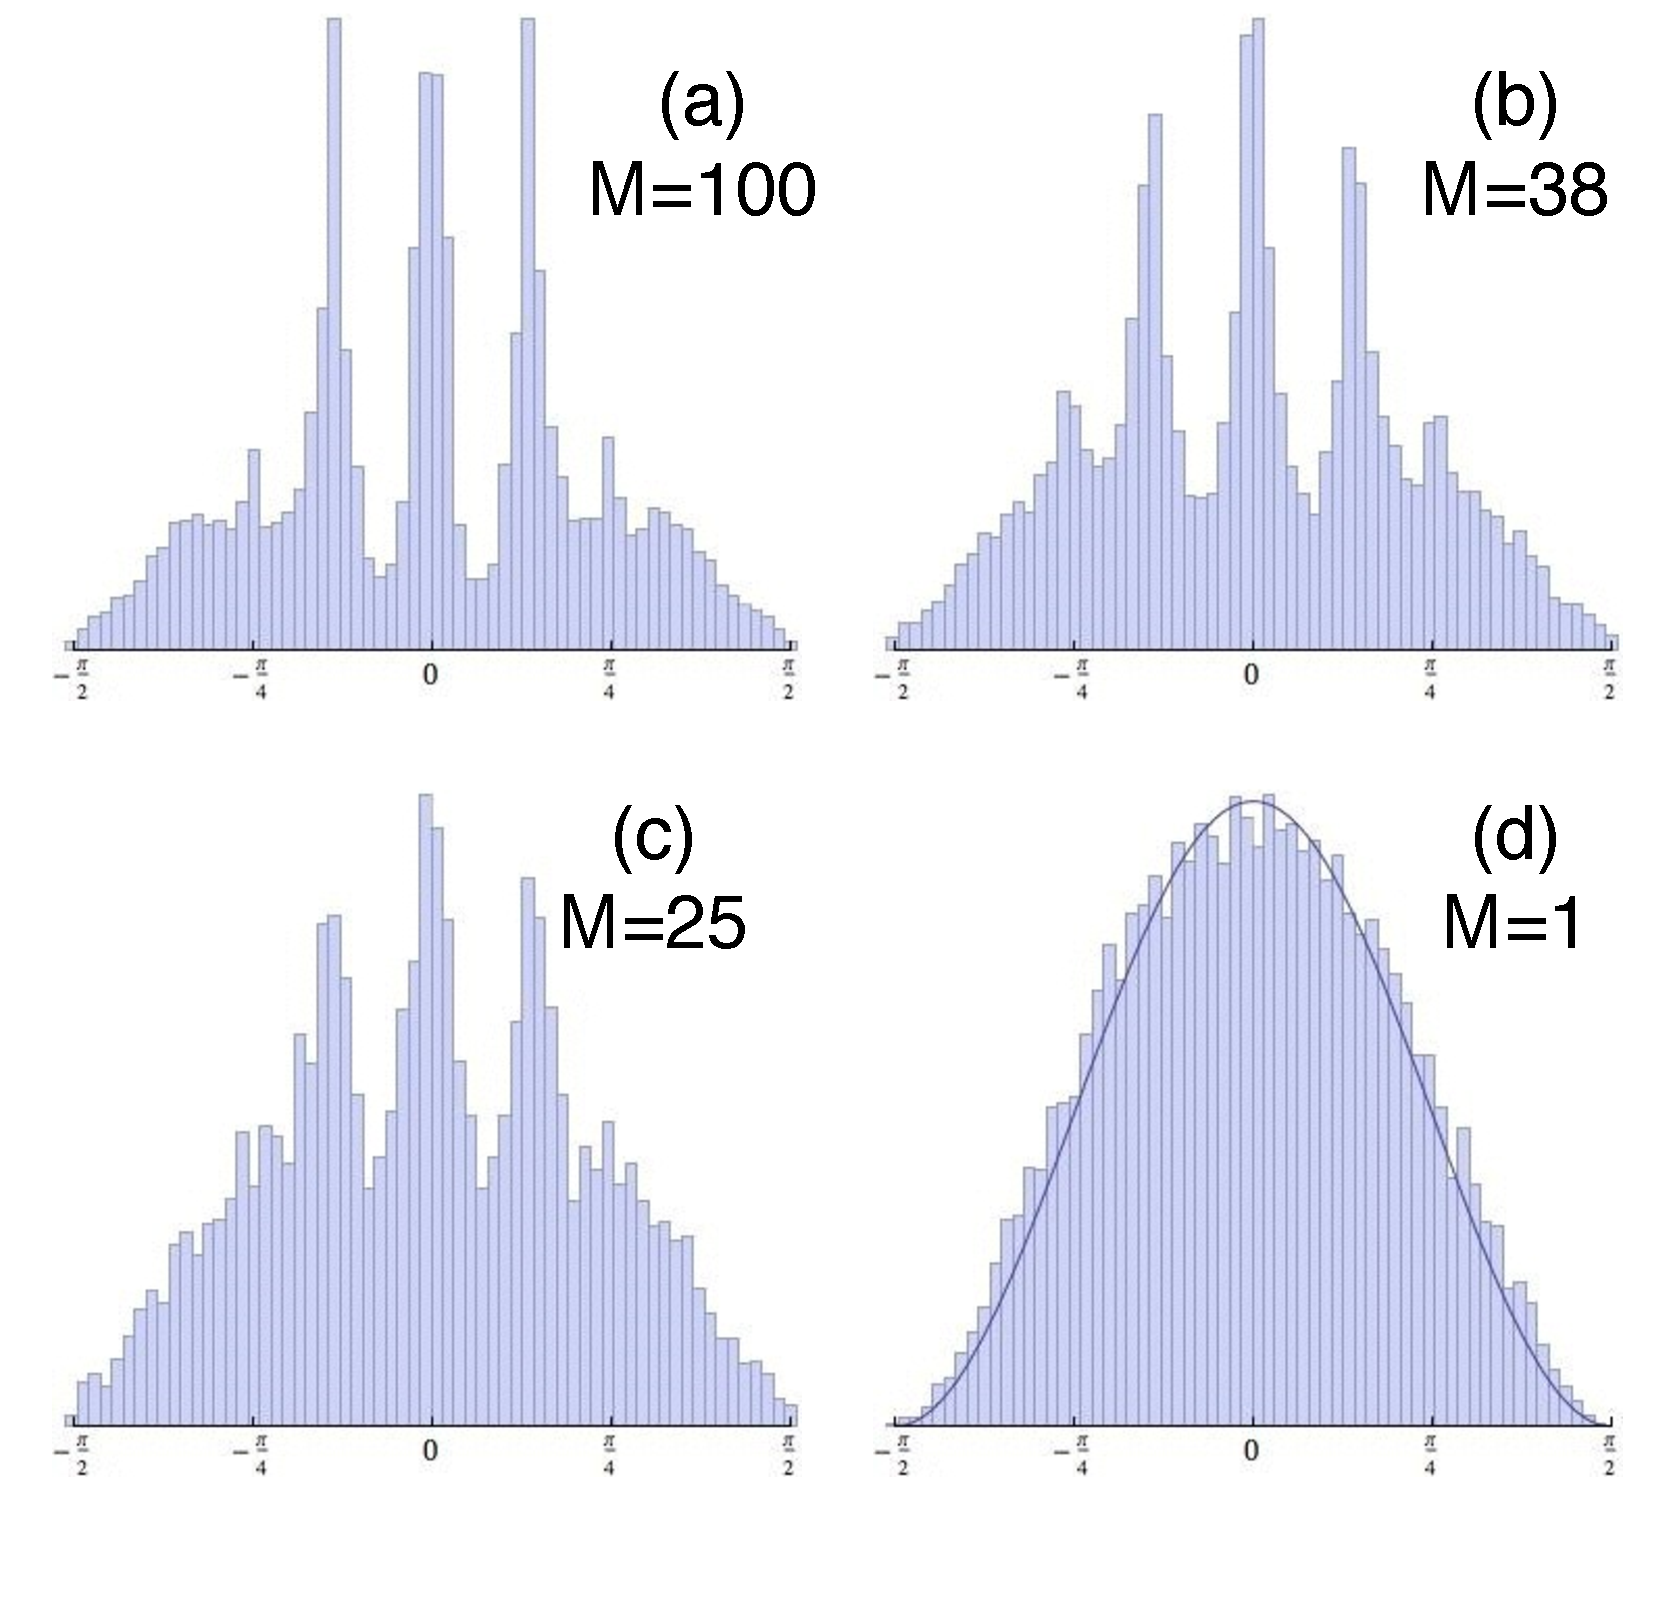
\includegraphics[width=1\linewidth]{Graphics/CombinedGraphics/DoubleSlitVisibilityHistograms}
\caption{Histogram indicating the angle of Bohmian trajectories from two slits a distance 5mm apart with a gaussian slit width of width 1mm at a distance of 70mm from the origin.  Histogram for many droplet trajectories from two slits a distance 5mm apart with a slit width of width 1mm at a distance of 70mm from the origin.  The memory has been changed to $300$ which results in a visibility of $0.8 \pm 0.1$.  The memory has been changed to $100$ which results in a visibility of $0.8 \pm 0.1$.}
\label{fig:DoubleSlitVisibilityHistograms}
\end{figure}

[Figure should be histogram for bohmian case, two visibility histograms, and then the visibility plot.]

\begin{figure}[ht]
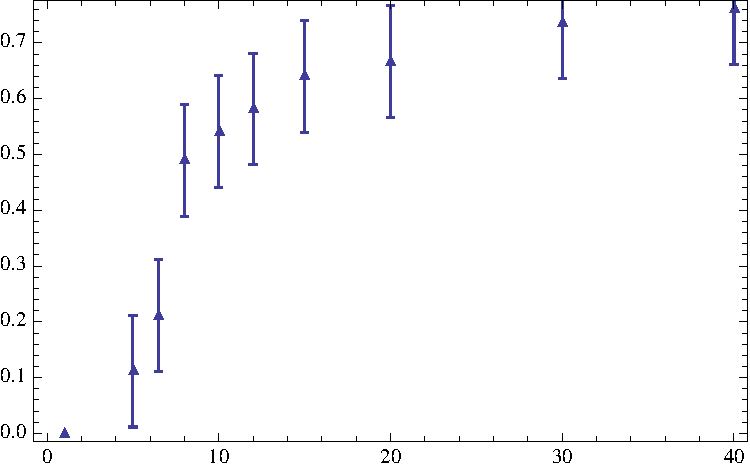
\includegraphics[width=1\linewidth]{Graphics/VisibilityPlot}
\caption{The visibility of the interference pattern as a function of the memory parameter for the single slit(blue) and the double slit (red).}
\label{fig:VisibilityPlot}
\end{figure}

[Double slit for crossings]

We now compute the trajectories for the double slit experiment using the same initial conditions as the single slit above.  The results are shown in Fig.~\ref{fig:DoubleSlitDensitiesAndTrajectories}-D can be contrasted against the trajectories in Fig.~\ref{fig:DoubleSlitDensitiesAndTrajectories}-C, which are the result of the quantum wavefunction and Bohm's quantum force.  One of the tenants of Bohmian trajectories is that the trajectories are forbidden cross each other.  It is obvious that the trajectories in Fig.~\ref{fig:DoubleSlitDensitiesAndTrajectories}-D have no such reluctance.  However, if we look at the matching histogram given by Fig.~\ref{fig:DoubleSlitVisibilityHistograms}-B we note that the interference pattern that builds gives similar results to that of the quantum case.  As with the single slit the experiment gives similar results to the quantum case.

[Give uncertainties for the visibilities and ground the equation for visibility in references.]

To further make comparisons with quantum mechanics we can look at, as a function of the memory parameter, the visibility, $V$, of the interference pattern in the vicinity of the central peak defined by
\begin{align}
V = \frac{I_{max}-I_{min}}{I_{max}+I_{min}}
\end{align}
where $I_{max}$ is the hight of the central peak and $I_{min}$ is the hight of the first minima[cite].  The paths in Fig.~\ref{fig:DoubleSlitDensitiesAndTrajectories}-B and the histogram in Fig.~\ref{fig:DoubleSlitVisibilityHistograms}-B assume a very high memory parameter but realistically, after the droplet has passed through a slit, the interference pattern will begin to degrade.  If we plot the histogram for several values of the memory parameter, Figs.~\ref{fig:DoubleSlitVisibilityHistograms}-C,D, we note that the visibility is proportional to the memory parameter.  In quantum mechanics the visibility reduces as a function of the which path information.  We can rephrase this, in the light of wave-particle duality, to say that the more particle-like the initial state is, the less visibility there will be.  We can make this same analogy with the bouncing droplet system by observing that the lower that the memory parameter is, the weaker the accumulated effective wave function and the weaker the force on the droplet.  With a weaker effective potential the droplet behaves more like a classical particle.

[Memory of 1?]

\section{Discussion}

[Indicate that our model may be able to explain experimental results]

It should be noted that, while it is known that a walking droplet has a constant velocity in the absence of any potentials, it is unclear if the magnitude of the velocity must remain constant when the droplet enters an area where the effective wavefunction has an influence on the droplet like after a double slit.  The model above assumes that the droplet can take any velocity after the double slit although the damping factor will make extremely large velocities unlikely.

We would like to note that the system as modeled above is very sensitive to initial conditions.  One problematic initial condition is the initial speed of the droplet after it passes through one of the slits.  In Fig.~\ref{fig:DoubleSlitDensitiesAndTrajectories}-B,C,D the velocity was set equal to the velocity of the effective wave function, a reasonable assumption assuming the passage through the slit has a negligible influence on the droplets velocity before the slit.  If however the passage through the slit reduces the velocity the trajectories will change significantly. [Actually show that the visibility is reduced] [Also maybe note that the distribution of velocities from the slit is cosine distributed and this may not be realistic], [Also note that if the particle does not start far from the slit then even with a high memory parameter, the wavefunction behind the slit may not build up properly.]

We could make a effort to make some relation of the wave equation to the Schr\"odinger equation as has been done by Sbitnev[CITE], but we question the usefulness of this.  The unique properties of quantum mechanics due to the Schr\"odinger equation cannot be readily transposed to the droplet system just by equating the wave equation governing the liquid medium to Schr\"odingers equation.  As we stated in the introduction the guiding equation must also be considered and while the Bohmian quantum force can be derived from Schr\"odingers equation and therefore preserve the unique properties the Schr\"odinger equation imparts, the guiding equation of the bouncing droplet system does not flow from Schr\"odingers equation.  Further, we are not expecting to find direct mathematical analogues to quantum mechanics.  The bouncing droplet system is, after all, completely classical.  What we are exploring are the behavioral analogues which frees us from duplicating the Schr\"odingers equation as the wave equation for the buncing droplet system.

\section{Think like Bohm}

One of the tenants of Bohmian mechanics is that the particle has no properties besides its position and the wave function is completely determined by the experimental apparatus.  For example, in the quantum double slit system, the experiment is constructed in such a way that the photons have an equal probability of passing through either slit.  It is this experimental construction which defines the wavefunction in the Bohmian interpretation.  This has not been the approach taken so far by the various bouncing droplet experiments.  In those experiments the droplet was the source of the wavefunction and not the experiment.  This is more akin to de Broglie's original dual solution theory, as has been mentioned by Couder[CITE], in which the guided particle has an oscillatory property similar to a de Broglie wavelength.  In the experiments so far the droplet has been responsible for the wave that will then interact with the experiment (for example a double slit) and then determine the trajectory of the particle.  We submit that there is no need for this to be the case and that we are only holding on to this paradigm for historical reasons.

It is the case that the non-coalescence of the droplet only happens when the bath is vibrating near the faraday threshold.  Near this threshold the bouncing of the droplet causes Faraday waves to be excited.  The closer we come to the Faraday threshold the longer these excited waves remain active.  It has been these waves that have been observed by experiment to be responsible for the analogous quanta effects that we have seen so far.  There is, however, nothing special about these excited waves. The droplet only requires these excited waves to exist in the immediate vicinity of the droplet in order to maintain the bouncing.  In fact, we do not actually need these specific excited waves to observe pilot wave behavior.  It should be obvious that any wave that intersects with the droplet, either produced by the droplet itself or induced externally, will effect the droplet.  This realization then gives us the freedom to approach the system in a more Bohmian manner and separate the excited waves from the droplet and replace them with an induced wave that we define by the experiment we wish to perform.

We have shown through intuition and approximation that in the case of the double slit experiment the complex excited waves can combine in such a way that they develop an interference pattern behind the slit.  This analysis relies on assumptions and approximation which, while being reasonable, are unnecessary.  We can instead induce whatever wave we choose, separate from the droplet, to give us any wave function that we desire and avoid many complications.  In the case of the double slit experiment if we induce a monochromatic plane wave that travels to the slits, the interference pattern that develops after the slits is obvious and independent of the droplet.  The interaction with the droplet is therefore much simplified and much more controllable.  An obvious way in which it is more controllable is that we now have the freedom to choose any wavelength for the induced pilot wave.  If we choose only the waves excited by the droplet we are limited to the frequency which can take only one value and is dependent on the single frequency of the vibrator.  Additionally since we are not relying on the bath to store the effect of each bounce we can be independent of the memory parameter.  In fact, it may be beneficial to work in the low memory regime so that the excited waves do not strongly interfere with the induced waves.
%
%Having happened upon this extraordinary system in which we observe pilot wave dynamics analogous to a quantum system by separating of a macroscopic classical wave from a macroscopic particle we can imagine other quantum analogous systems possibly even more classical (larger) than the bouncing droplet system.  Consider, for example, an ocean wave impinging on a slit and a surfer riding that wave.  The water waves would produce an interference pattern behind the slit and if we assume that the surfers guiding equation is similar to the hydrodynamic guiding equation then the passage of many surfers would lead to an interference pattern of surfers on the beach.  These quantum surfers are therefore another analogue of quantum particles.

\section{Conclusion}

The behavior of the bouncing droplet system we have explored obviously does not flow from the mathematical foundations of quantum mechanics.  It is not linear, etc...  It does however have analogous behavior we usually only associate with quantum mechanics.  The superposition principle holds, probability is preserved in some sense. etc...  It is therefore reasonable to ask what ingredients are needed to see this kind of quantum behavior in other systems.  Looking at the droplet system it would seem that a wave equation and a guiding equation are all thats necessary.  To that end two people bouncing on a trampoline can be considers a quantum analogue.  The bouncers have an effective wavefunction, given by the shape of the trampoline surface.  The wavefunction is non-local.  There is a guiding equation given by the force the rebound of the trampoline exerts upon the bouncers.  There is interference.  There is even an analogue to the Pauli exclusion principle as two bouncers cannot be in the same place at the same time.  We are of the opinion that many other quantum analogue systems can be envisioned.

\begin{acknowledgments}
This work was financially supported by the Actions de Recherches Concert\'ees (ARC) of the Belgium Wallonia-Brussels Federation under contract No.~12-17/02.
\end{acknowledgments}

\bibliography{Biblio}
\end{document}  